\shorthandoff{"}
\chapter{Verwandte Arbeiten}
\label{ch:verwandteArbeiten}
In der Literatur verfolgten bereits einige Publikationen den Anspruch, Empfehlungssysteme zur automatisierten Bestimmung des \acp{PJFit} zu entwickeln. Aus dem Blickwinkel der Berufs- und Organisationspsychologie handelt es sich bei diesem Begriff um eine Version des \acp{PEFit}, bei welcher für die Umgebung die Aspekte einer Stelle betrachtet werden \cite[S. 1ff.]{edwards:1991}\cite[S. 3]{malinowski:2006}. Jedoch bezogen sich einige Forscher in ihren Veröffentlichungen nicht auf das in Kapitel \ref{ch:personEnvironmentFit} vorgestellte Konzept der Psychologie. Obwohl der Begriff des \acp{PJFit} verwendet wurde, bestimmten die Wissenschaftler die Kongruenz häufig ausschließlich auf der Ebene des Anforderungen-Fähigkeiten Fits. Dieser Sachverhalt ist beispielsweise bei \textcite[S. 1ff.]{luo:2019}, \textcite[S. 1ff.]{qin:2018} und \textcite[S. 1ff.]{personJobFit:2018} zu beobachten.

\section{Nicht auf dem P-E Fit basierende Systeme}
\label{ch:verwandteArbeiten:nichtAufDemPEFitBasierend}
\textcite[S. 1, Z. 1f.]{personJobFit:2018} definierten den \ac{PJFit} als den "Prozess, bei dem das richtige Talent mit der richtigen Stelle zusammengeführt wird, indem die Talentkompetenzen identifiziert werden, welche für die Stelle erforderlich sind."\footnote{"process of matching the right talent for the right job by identifying talent competencies that are required for the job." - \textcite[S. 1, Z. 1f.]{personJobFit:2018}} Dementsprechend implementierten \textcite[S. 1ff.]{personJobFit:2018}, wie auch \textcite[S. 1ff.]{luo:2019} und \textcite[S. 1ff.]{qin:2018}, ein neuronales Netz, welches voraussagte, ob eine Person aufgrund ihrer Qualifikationen für eine Stelle geeignet ist. Hierfür bereiteten sie unstrukturierte Stellenausschreibungen und Lebensläufe strukturiert auf. Anschließend nutzten die drei Forschergruppen die gewonnenen Daten, um anhand verschiedener Verfahren vorauszusagen, ob die Fähigkeiten der Kandidaten die Anforderungen der offenen Stellen erfüllen \cite[S. 1ff.]{luo:2019}\cite[S. 1ff.]{qin:2018}\cite[S. 1ff.]{personJobFit:2018}.%Somit implementierten diese Wissenschaftler ausschließlich Lösungen zur Bestimmung des Anforderungen-Fähigkeiten Fits.

Empfehlungssysteme, welche neben den Präferenzen der Personalverantwortlichen an die Fähigkeiten potentieller Mitarbeiter auch die Wünsche der Kandidaten berücksichtigen, bezeichneten \textcite[S. 4]{malinowski:2006} als bilaterale Empfehlungssysteme. Solche Anwendungen beziehen neben dem Anforderungen-Fähigkeiten Fit folglich auch die Bedürfnisse-Angebote Kongruenz in den Vorschlagsprozess ein. Verschiedene Forschergruppen aus dem Umfeld von \textcite[S. 1ff.]{malinowski:2006} entwickelten mehrere bilaterale Recommender Engines, welche in unterschiedlichen Publikationen vorgestellt wurden. Dabei bezogen sich die Wissenschaftler auf das in Kapitel \ref{ch:personEnvironmentFit} vorgestellte Konzept des \acp{PEFit} \cite[S. 4ff.]{keim:2007}\cite[S. 3f.]{keim:2005}\cite[S. 2ff.]{malinowski:2005}\cite[S. 3f.]{malinowski:2006}\cite[S. 3ff.]{malinowski:2008}. Alle diese Implementierungsmethoden basieren auf einem von \textcite[S. 1ff.]{faerber:2003} vorgestellten Empfehlungssystem.

\section{Auf dem P-E Fit basierende bilaterale Systeme}
\label{ch:verwandteArbeiten:aufDemPEFitBasierendeBilateraleSysteme}

\subsection{Unilaterales Empfehlungssystem für Personalsachbearbeiter}
\label{ch:verwandteArbeiten:aufDemPEFitBasierendeBilateraleSysteme:grundlegendesEmpfelungssystem}
\textcite[S. 4ff.]{faerber:2003} entwickelten eine Recommender Engine zur Empfehlung von Personen für offene Stellen in Unternehmen. Dabei verfolgten sie einen hybriden, nicht-bilateralen Ansatz. Dieser ist in Abbildung \ref{fig:verwandteArbeiten:abb1} modelliert.

\begin{figure}[h]
	\centering
	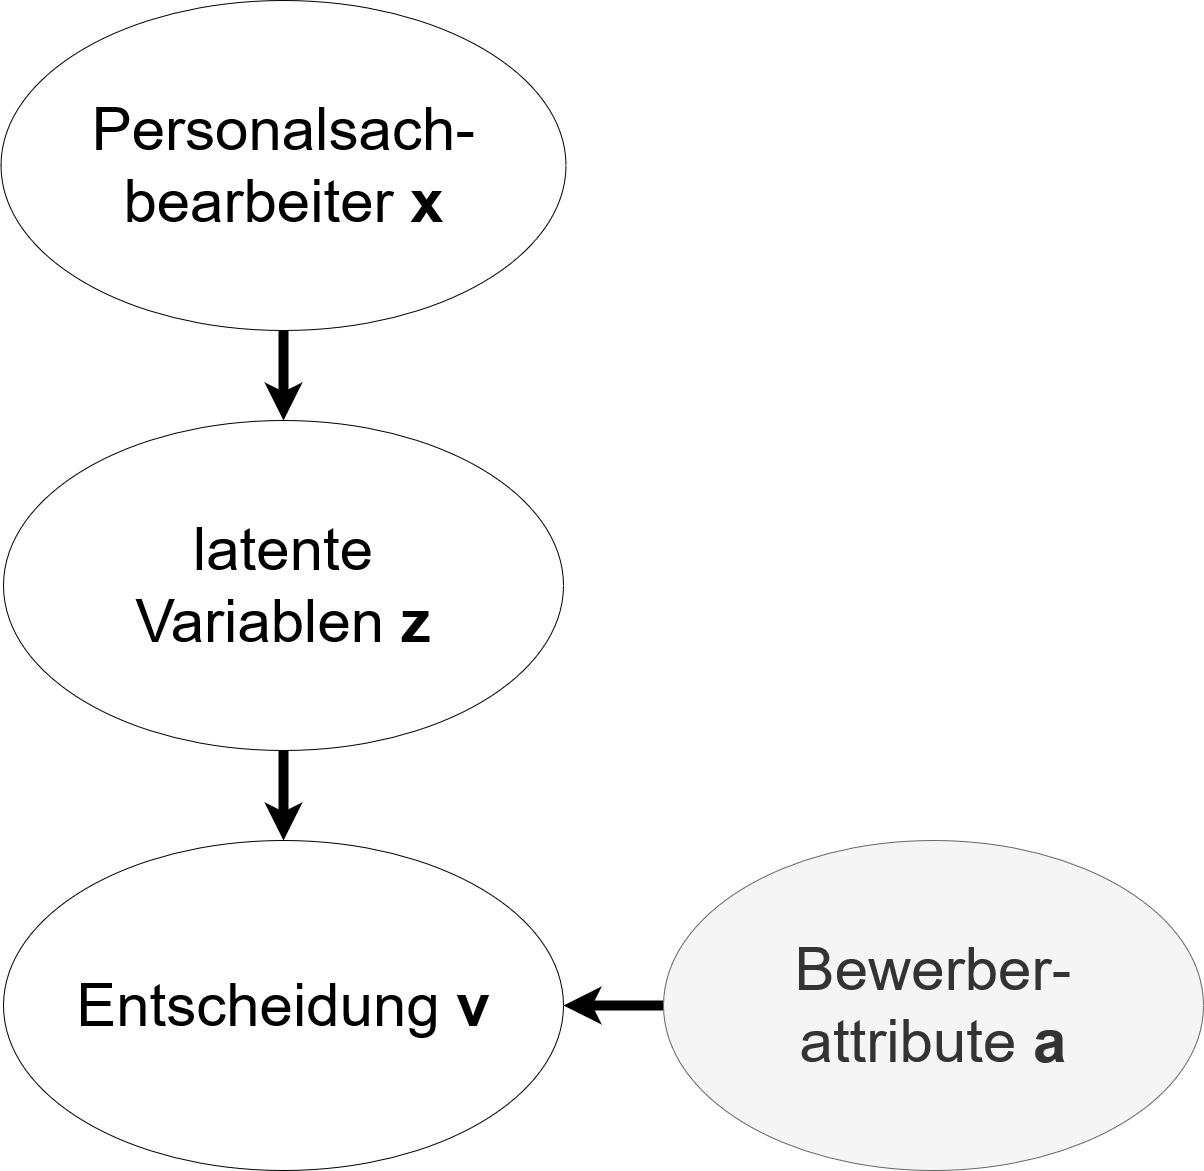
\includegraphics[width=0.5\textwidth]{gfx/faerber.jpg}
	\caption[Modell des hybriden Empfehlungssystems für Personalsachbearbeiter]{Modell des hybriden Empfehlungssystems für Personalsachbearbeiter\\
	(Eigene Darstellung in Anlehnung an \cite[S. 8]{faerber:2003})}
	\label{fig:verwandteArbeiten:abb1}
\end{figure}

In Abbildung \ref{fig:verwandteArbeiten:abb1} steht $a$ für Attribute aus dem Lebenslauf eines Bewerbers, wie dem Namen seiner Hochschule oder der Abschlussnote seines Studiums \cite[S. 4]{malinowski:2006}. Variable $x$ symbolisiert einen Personalsachbearbeiter mitsamt eines Stellenprofils, welches dieser besetzen soll. Dessen Entscheidung, ob ein Bewerber für die Tätigkeit qualifiziert ist oder nicht, wird über den booleschen Wert $v$ ausgedrückt \cite[S. 6ff.]{faerber:2003}.

\textcite[S. 4ff.]{faerber:2003} bestimmten aus diesen Faktoren ein latentes Variablenmodell. Hierbei wurden bekannte Entscheidungen eines Personalsachbearbeiters hinsichtlich der Eignung von Bewerbern für eine Stelle erfasst. Aus diesen wurden nicht direkt messbare Variablen $z$ abgeleitet, welche dessen Beurteilungen beeinflussten. Über die latenten Variablen $z$ und die Attribute $a$ bestimmten die Autoren Wahrscheinlichkeiten, mit welchen der Personalsachbearbeiter die vorliegenden Attribute der Kandidaten als qualifiziert oder unqualifiziert bewerten würde \cite[S. 4ff.]{faerber:2003}.

Diesen Empfehlungsansatz nutzten \textcite[S. 4f.]{malinowski:2006} als Grundlage für ein neues Empfehlungssystem. Die Wissenschaftler stellten eine Anwendung vor, welche neben den Präferenzen der Personalsachbearbeiter auch die Wünsche der Kandidaten berücksichtigte.

\subsection{Einbeziehung von Präferenzen der Kandidaten}
\label{ch:verwandteArbeiten:aufDemPEFitBasierendeBilateraleSysteme:einbeziehungKandidaten}
Um neben den Präferenzen der Personalsachbearbeiter auch die Wünsche der Kandidaten in den Vorschlagsprozess einzubeziehen, erweiterten \textcite[S. 4f.]{malinowski:2006} das von \textcite[S. 4ff.]{faerber:2003} entwickelte Empfehlungssystem um eine zusätzliche Komponente für Stellensuchende. Diese orientierte sich ebenfalls am Aufbau von Abbildung \ref{fig:verwandteArbeiten:abb1}. Bei der neuen Komponente stand $x$ für den Kandidaten und $a$ für die Attribute der Stellenausschreibung. Auch hier bestimmten die Forscher latente Variablen $z$, welche sie über vergangene Stellenprofil-Bewertungen von Studenten ermittelten. Über diese sagten sie voraus, mit welcher Wahrscheinlichkeit ein Kandidat eine Stelle als passend zu seinen Präferenzen bewerten würde \cite[S. 4f.]{malinowski:2006}.

Bei einer Evaluation des Systems stellten \textcite[S. 6f.]{malinowski:2006} fest, dass die Ergebnisse der Komponente zur Empfehlung von Kandidaten nahezu vergleichbar zur manuellen Auswahl eines menschlichen Personalsachbearbeiters waren. Auch beim Stellenempfehlungssystem kamen sie zu der Erkenntnis, dass die Ergebnisse bis auf wenige Ausnahmen vergleichbar zur manuellen Selektion der Kandidaten waren.%\textcite[S. 7]{keim:2007} bestätigte ebenfalls, dass beide Empfehlungsmodule eine hohe Genauigkeit aufweisen konnten.

Zum Vorgehen von \textcite[S. 3ff.]{malinowski:2006} ist festzustellen, dass das bilaterale Empfehlungssystem ursprünglich in Anlehnung an das Konzept des \acp{PEFit} entwickelt wurde. Dabei sollten sowohl Präferenzen von Personalsachbearbeitern als auch Wünsche von Stellensuchenden berücksichtigt werden. Allerdings ist es in der vorgestellten Anwendung nur möglich, entweder zu den Präferenzen von Personalsachbearbeitern passende Kandidaten oder mit den Wünschen von Bewerbern kompatible Stellen zu ermitteln. Es ist nicht vorgesehen, Kandidaten für Positionen zu empfehlen und dabei gleichzeitig die Präferenzen von Bewerbern und Personalsachbearbeitern zu berücksichtigen. Daher ist kritisch anzumerken, dass die Anwendung von \textcite[S. 1ff.]{malinowski:2006} zwar die Präferenzen beider Parteien einbezog, dieses Vorgehen aber nicht der Theorie des \acp{PEFit} entspricht.

Ein Empfehlungssystem, welches das Konzept des \acp{PEFit} dagegen erfüllte, stellten \textcite[S. 1ff.]{malinowski:2005} in einer anderen Publikation vor.

\subsection{System zur bilateralen Vertrauensbestimmung}
\label{ch:verwandteArbeiten:aufDemPEFitBasierendeBilateraleSysteme:bilateraleVertrauensbestimmung}
\textcite[S. 1]{malinowski:2005} präsentierten eine Recommender Engine, welche Personen für Teams vorschlagen sollte. Dabei berücksichtigten sie die Präferenzen von Personalsachbearbeitern hinsichtlich der fachlichen Eignung der Kandidaten. Außerdem beachteten sie die Wünsche von Teammitgliedern und potentiellen Kandidaten bezüglich der persönlichen Zusammenarbeit.

Das System von \textcite[S. 4ff.]{malinowski:2005} sah es in einem ersten Schritt vor, das Verfahren von \textcite[S. 8ff.]{faerber:2003} aus Kapitel \ref{ch:verwandteArbeiten:aufDemPEFitBasierendeBilateraleSysteme:grundlegendesEmpfelungssystem} anzuwenden. Damit bestimmten die Wissenschaftler aus allen verfügbaren Kandidaten die $N$ fachlich geeignetsten Personen passend zu den Präferenzen des Personalsachbearbeiters hinsichtlich des zu besetzenden Stellenprofils. Diese $N$ Kandidaten dienten als Eingabe für eine weitere Komponente, über welche die Forscher das gegenseitige Vertrauen zwischen diesen Personen und den bereits vorhanden Teammitgliedern berechneten. Um dieses zu bestimmen, nutzten die Autoren drei separate Ansätze, welche in Abbildung \ref{fig:verwandteArbeiten:abb2} dargestellt sind \cite[S. 4ff.]{malinowski:2005}. Sie wurden auch in den Publikationen von \textcite[S. 5ff.]{keim:2005} und \textcite[S. 6ff.]{malinowski:2008} behandelt.

\begin{figure}[h]
	\centering
	
	\subfloat[Transitive Beziehung]{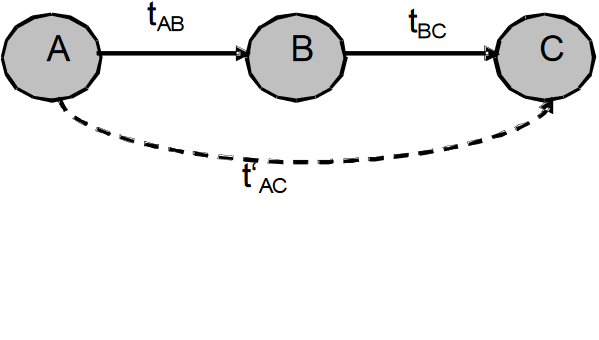
\includegraphics[width = 0.33\textwidth]{gfx/trustmodelA.png}}
	\subfloat[Kollaboratives Filtern]{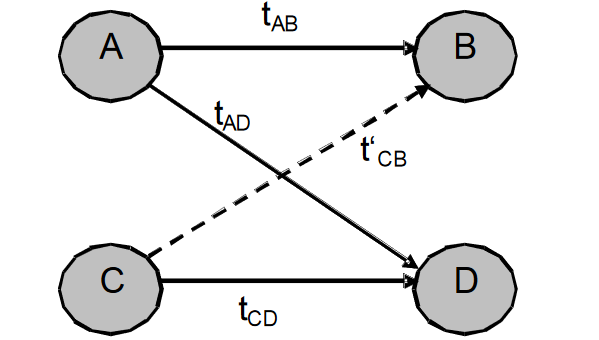
\includegraphics[width = 0.33\textwidth]{gfx/trustmodelB.png}}
	\subfloat[Ähnlichkeitsberechnung über latente Variablen]{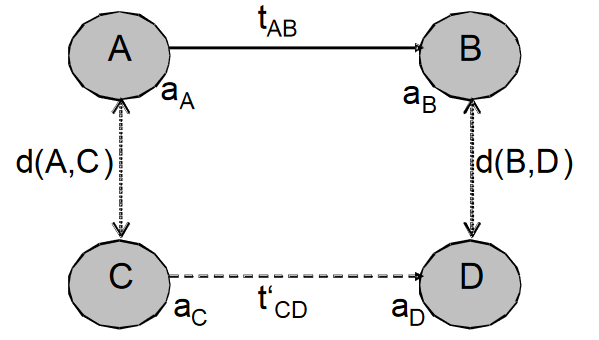
\includegraphics[width = 0.33\textwidth]{gfx/trustmodelC.png}}
	
	\caption[Ansätze zur Berechnung des Vertrauens zwischen potentiellen Teammitgliedern]{Ansätze zur Berechnung des Vertrauens zwischen potentiellen Teammitgliedern \cite[S. 5]{malinowski:2005}}
	\label{fig:verwandteArbeiten:abb2}
\end{figure}

Die Anwendung der ersten beiden Ansätze (a) und (b) zur Vorhersage des Vertrauens zwischen potentiellen Teammitgliedern aus Abbildung \ref{fig:verwandteArbeiten:abb2} setzt laut \textcite[S. 4ff.]{malinowski:2005} voraus, dass bekannte Vertrauensbewertungen von Teamkollegen vorhanden sind. Diese können den Wissenschaftlern zu Folge beispielsweise über Fragebögen ermittelt werden.

Bei Ansatz (a) nahmen \textcite[S. 5f.]{malinowski:2005} an, dass eine Vertrauensbeziehung über Multiplikation berechnet werden kann, wenn transitiv eine Verbindung zwischen zwei Personen besteht. Zur Berechnung der Vertrauensbeziehung $t'_{AC}$ von Person A zu Person C in Abbildung \ref{fig:verwandteArbeiten:abb2} (a), wendeten die Wissenschaftler Formel \ref{frml:verwandteArbeiten:formel1} an \cite[S. 6]{malinowski:2005}.
\begin{equation}
	t'_{AC} = t_{AB} * t_{BC}
	\label{frml:verwandteArbeiten:formel1}
\end{equation}
Ansatz (b) in Abbildung \ref{fig:verwandteArbeiten:abb2} zeigt die Berechnung des Vertrauens zwischen zwei Personen über speicherbasiertes kollaboratives Filtern, wie es in Kapitel \ref{ch:empfehlungssysteme:cf} vorgestellt wurde. Hierbei nutzten die Wissenschaftler die Ähnlichkeit zwischen den Personen A und C, um das Vertrauen zwischen den Personen C und B vorherzusagen \cite[S. 6]{malinowski:2005}.

Das dritte Verfahren (c) beruhte auf der Annahme, dass sich Personen stark vertrauen würden, wenn sie ähnliche persönliche Präferenzen teilen. Unter dieser Prämisse erstellten \textcite[S. 6f.]{malinowski:2005} ein latentes Variablenmodell vergleichbar zum Verfahren aus Kapitel \ref{ch:verwandteArbeiten:aufDemPEFitBasierendeBilateraleSysteme:einbeziehungKandidaten}. Über dieses bestimmten sie für jedes Teammitglied diejenigen latenten Variablen, welche für dieses bei der Bewertung vergangener Stellen besonders wichtig waren. Die ermittelten latenten Variablen und die gemeinsam bewerteten Stellenprofile nutzten die Forscher, um über die Ähnlichkeit zwischen Personen auf deren gegenseitiges Vertrauen zu schließen \cite[S. 6f.]{malinowski:2005}.

Das in den drei Ansätzen (a), (b) und (c) bestimmte Vertrauen zwischen bestehenden Teammitgliedern und potentiellen Kandidaten aggregierten \textcite[S. 7ff.]{malinowski:2005} unter Berücksichtigung der Anzahl gemeinsam bewerteter Stellenprofile zu einer finalen Vertrauensbewertung.

Im letzten Schritt des Systems errechneten \textcite[S. 9f.]{malinowski:2005} aus den Vorschlägen der $N$ Kandidaten, welche die höchste Eignung für die Präferenzen des Personalsachbearbeiters aufwiesen und den ermittelten Vertrauensbewertungen eine gemeinsame Ergebnisliste. Hierzu wendeten sie Formel \ref{frml:verwandteArbeiten:formel2} an \cite[S.10]{malinowski:2005}.
\begin{equation}
	R' = \alpha * t'_{M*y} * (1-\alpha) * r'_{x,y,v}
	\label{frml:verwandteArbeiten:formel2}
\end{equation}
In Formel \ref{frml:verwandteArbeiten:formel2} steht $t'_{M*y}$ für die Liste der Vertrauensbeziehungen und $r'_{x,y,v}$ für die fachlichen Bewertungen der Kandidaten. Für $\alpha$ setzten \textcite[S. 4ff.]{malinowski:2005} den Wert 0.5 ein. Kritisch merkten sie zu Formel \ref{frml:verwandteArbeiten:formel2} an, dass diese noch nicht optimal sei und weiterer Forschung bedarf \cite[S. 9]{malinowski:2005}.

Eine Evaluation des Gesamtsystems konnte in der Literatur nicht identifiziert werden. In der Publikation von \textcite[S. 13ff.]{malinowski:2008} findet sich lediglich eine Validierung der Komponente zur Berechnung des Vertrauens zwischen Teammitgliedern und potentiellen Kandidaten. Hierbei kamen die Wissenschaftler zu der Erkenntnis, dass deren System eine höhere Genauigkeit als eine zufällige Vorhersage aufweisen konnte. Allerdings merkten die Forscher an, dass ihre Testgruppe mit 21 Teilnehmern zu klein sei, um signifikante Resultate zu erzielen \cite[S. 13ff.]{malinowski:2008}. Die Autoren validierten gemäß der Forschungsfrage dieser Master-Thesis jedoch nicht, ob die erwarteten Ergebnisse des \acp{PEFit} von deren Empfehlungssystem reproduziert werden konnten. Somit bleibt ungewiss, ob auf Seiten der Personalsachbearbeiter die erwartete Arbeitsleistung der vorgeschlagenen Kandidaten und aus Perspektive der Mitarbeiter die Zufriedenheit mit der Stelle und den Teamkollegen zunahm.

Die Berechnung der gegenseitigen Vertrauensbeziehungen zwischen bestehenden Teammitgliedern und potentiellen Kandidaten nutzte auch \textcite[S. 1ff.]{keim:2007}. Er präsentierte ein Framework, welches Personen in passende Projektteams einordnen und dabei sowohl Fähigkeiten als auch zwischenmenschliche Attribute berücksichtigen sollte \cite[S. 1ff.]{keim:2007}.

\subsection{Mehrschichtiges Framework}
\label{ch:verwandteArbeiten:aufDemPEFitBasierendeBilateraleSysteme:pjUndPtFit}
Das von \textcite[S. 5]{keim:2007} vorgestellte Framework ist in Abbildung \ref{fig:verwandteArbeiten:abb3} dargestellt. Es besteht aus drei Schichten.

\begin{figure}[h]
	\centering
	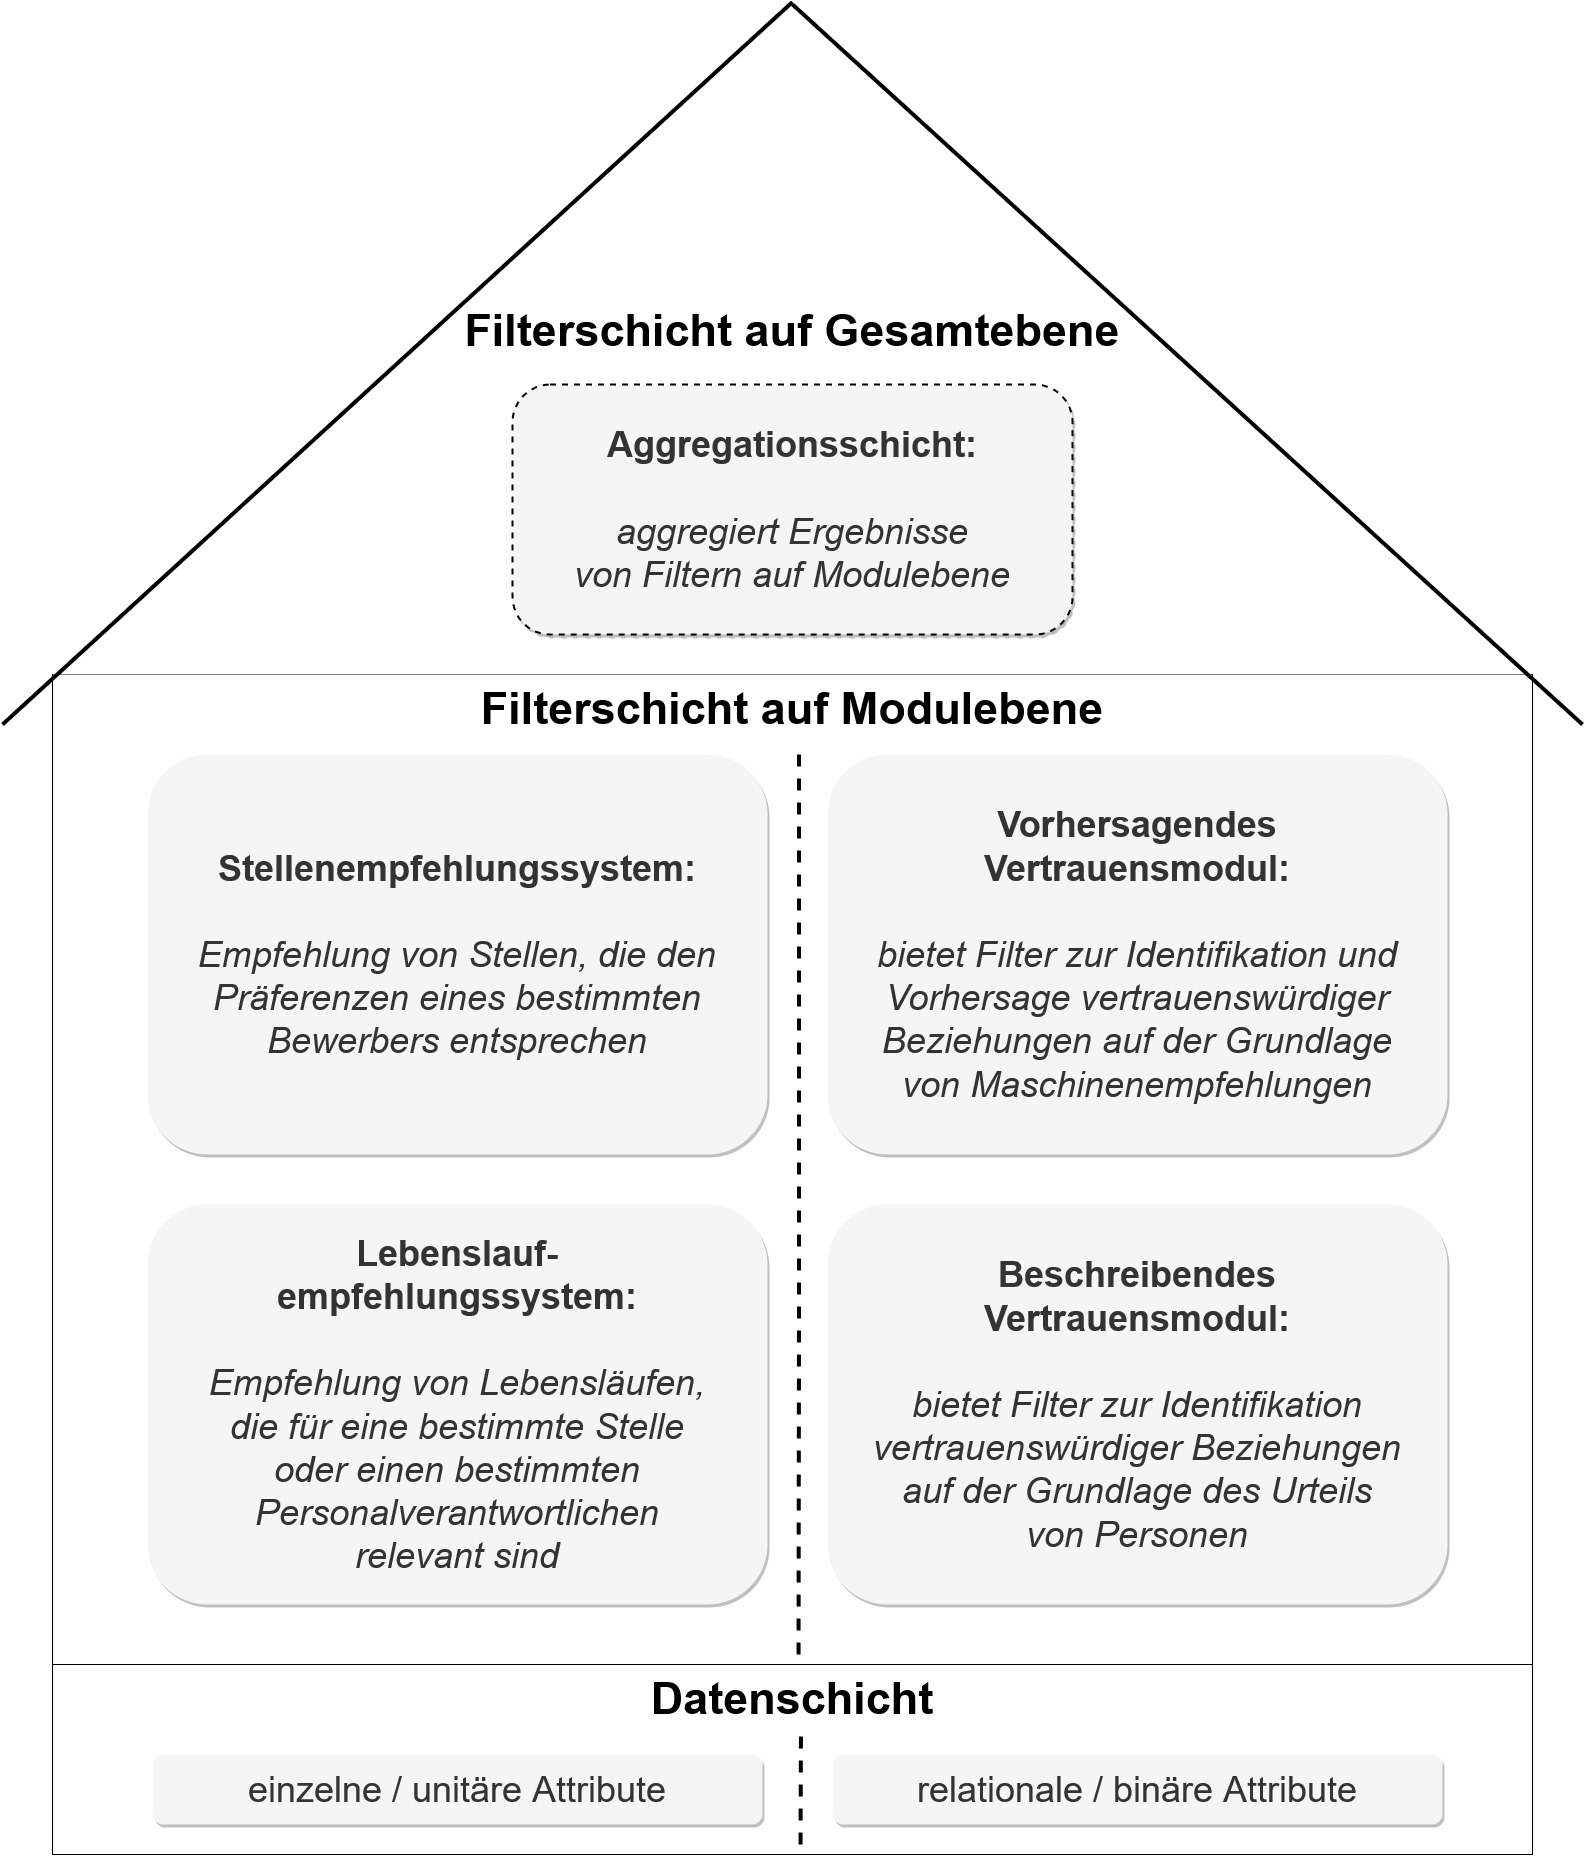
\includegraphics[width=1\textwidth]{gfx/keim-multilayer.jpg}
	\caption[Framework zur Einordnung von Personen in Projektteams]{Framework zur Einordnung von Personen in Projektteams\\
	(Eigene Darstellung in Anlehnung an \cite[S. 5]{keim:2007})}
	\label{fig:verwandteArbeiten:abb3}
\end{figure}

In Abbildung \ref{fig:verwandteArbeiten:abb3} ist zu erkennen, dass sich die mittlere Schicht des Frameworks von \textcite[S. 5ff.]{keim:2007} aus vier Komponenten zusammensetzt. Diese vier Module laden die Daten der untersten Schicht und filterten diese entsprechend ihrer Funktion. Dabei unterstützen die beiden auf der linken Seite abgebildeten Module die Stellen- bzw. Kandidatensuche und die Komponenten der rechten Seite erleichtern die Bestimmung geeigneter Teampartner \cite[S. 5]{keim:2007}.

Das Lebenslaufempfehlungssystem in Abbildung \ref{fig:verwandteArbeiten:abb3} entspricht von \textcite[S. 8ff.]{faerber:2003} entwickelten Anwendung \cite[S. 6]{keim:2007}, welche in Kapitel \ref{ch:verwandteArbeiten:aufDemPEFitBasierendeBilateraleSysteme:grundlegendesEmpfelungssystem} vorgestellt wurde. Beim Stellenempfehlungssystem handelt es sich um die von \textcite[S. 4ff.]{malinowski:2006} adaptierte Version des Lebenslaufempfehlungssystems, mit welcher Personen zu ihren Präferenzen passende Stellenausschreibungen ermitteln können \cite[S. 6]{keim:2007}. Dieses wurde in Kapitel \ref{ch:verwandteArbeiten:aufDemPEFitBasierendeBilateraleSysteme:einbeziehungKandidaten} behandelt. Das vorhersagende Vertrauensmodul entspricht dem in Kapitel \ref{ch:verwandteArbeiten:aufDemPEFitBasierendeBilateraleSysteme:bilateraleVertrauensbestimmung} behandelten Ansatz zur Vorhersage von Vertrauensbeziehungen zwischen potentiellen Teampartnern \cite[S. 8]{keim:2007}. Das beschreibende Vertrauensmodul erfasst explizit vergebene Vertrauensbewertungen von Teammitgliedern in Form einer Ontologie und repräsentiert diese optisch in Form eines Graphen. Über diese Darstellung können Anwender soziale Beziehungen durchsuchen und analysieren. Auf diese Weise sollen sie besser entscheiden können, mit welchen Personen sie eine Zusammenarbeit eingehen möchten \cite[S. 7]{keim:2007}.

Ähnlich zur Publikation von \textcite[S. 3ff.]{malinowski:2006} muss auch zur Veröffentlichung von \textcite[S. 5ff.]{keim:2007} kritisch bemerkt werden, dass der Forscher die Resultate der einzelnen Module nicht zu einem Ergebnis zusammenfasste. Die Implementierung der oben in Abbildung \ref{fig:verwandteArbeiten:abb3} dargestellten Aggregationsschicht, welche bilaterale Empfehlungen ermöglichen würde, ließ der Wissenschaftler offen \cite[S. 8]{keim:2007}.

\section{Wechselseitiges Empfehlungssystem zum Person-Job Fit}
\label{ch:verwandteArbeiten:nichtAufDemPEFitBasierendeBilateraleSysteme}
Neben den im vorherigen Kapitel \ref{ch:verwandteArbeiten:aufDemPEFitBasierendeBilateraleSysteme} vorgestellten Veröffentlichungen wurden bei der Literaturanalyse weitere Ansätze identifiziert, bilaterale Empfehlungssysteme zu implementieren. Die Autoren bezeichneten ihre Anwendungen jedoch nicht als bilateral, sondern als wechselseitig \cite[S. 1]{hong:2013b}\cite[S. 1]{wenxing:2015}.

Der Begriff der wechselseitigen Empfehlungssysteme wurde erstmals von \textcite[S. 1]{pizzato:2010} eingeführt, welche eine Recommender Engine im Bereich des Online-Datings entwickelten \cite[S. 1]{wenxing:2015}. Die Autoren verwendeten dabei die Bezeichnung der Wechselseitigkeit, da ihr System sowohl die Präferenzen des aktiven Nutzers als auch der potentiellen Partner gleichermaßen berücksichtigen sollte \cite[S. 1]{pizzato:2010}. In ihrer Publikation nannten \textcite[S. 3]{pizzato:2010} die Veröffentlichung von \textcite[S. 1ff.]{malinowski:2006} als verwandte Arbeit. Hierzu stellten sie fest, dass auch bilaterale Empfehlungssysteme die Präferenzen von zwei Parteien betrachten. Eine klare Unterscheidung zwischen bilateralen und wechselseitigen Empfehlungssystemen nahmen die Autoren jedoch nicht vor \cite[S. 3]{pizzato:2010}. Erst in einer späteren Publikation hielten \textcite[S. 8]{pizzato:2013} eindeutig fest, dass wechselseitig und bilateral zwei unterschiedliche Begriffe für dasselbe Konzept von Empfehlungssystemen sind.

Ein wechselseitiges Empfehlungssystem zum \ac{PJFit} stellten \textcite[S. 1ff.]{wenxing:2015} vor. Sie bezogen sich in ihrer Veröffentlichung nicht explizit auf das Konzept des \acp{PEFit}. Dennoch entwickelten die Autoren ein System zur Stellenbesetzung, welches sowohl Präferenzen von Stellensuchenden als auch Personalsachbearbeitern gleichermaßen in den Vorschlagsprozess einbezog. Wie in Abbildung \ref{fig:verwandteArbeiten:nichtAufDemPEFitBasierendeBilateraleSysteme:abb1} dargestellt, teilte die Anwendung die hinterlegten Informationen der beiden Nutzergruppen in die Kategorien Selbstbeschreibung und Präferenz \cite[S. 2]{wenxing:2015}.

\begin{figure}[h]
	\centering
	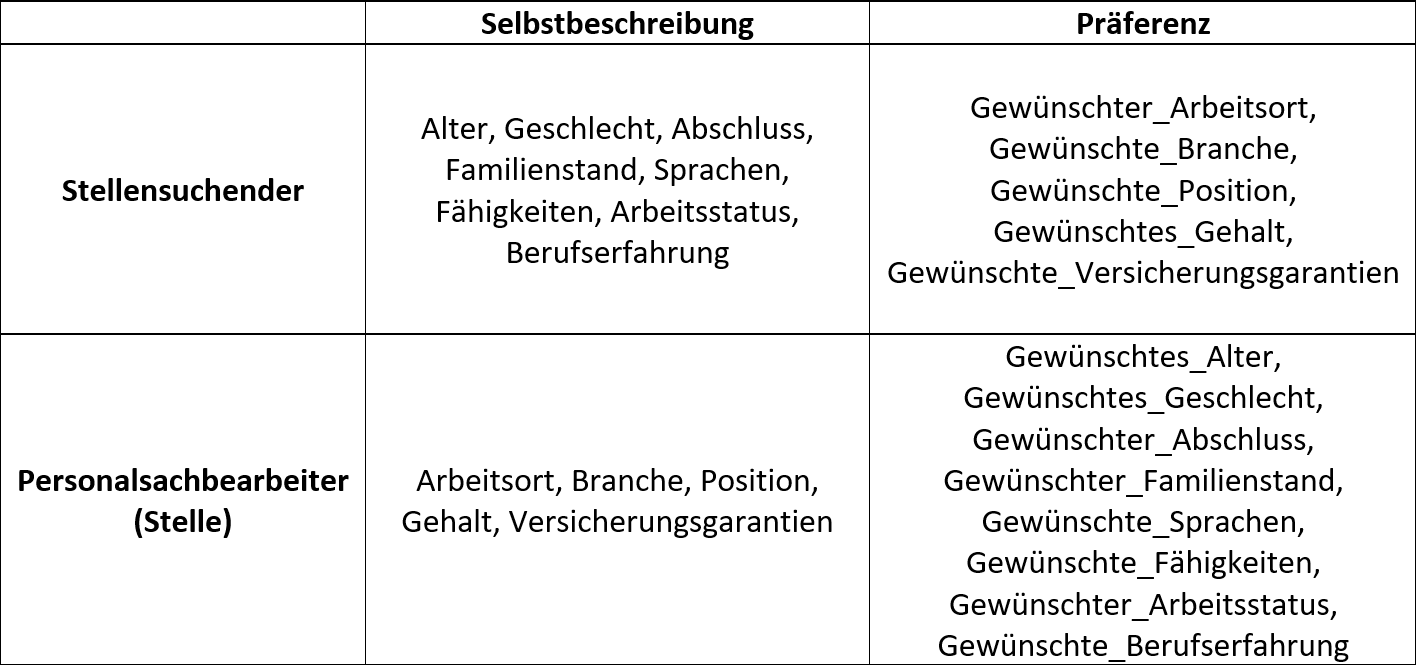
\includegraphics[width=1\textwidth]{gfx/hong-tabelle.png}
	\caption[Tabelle mit Merkmalskategorien des wechselseitigen Empfehlungssystems]{Tabelle mit Merkmalskategorien des wechselseitigen Empfehlungssystems\\
	(Eigene Darstellung in Anlehnung an \cite[S. 2]{wenxing:2015})}
	\label{fig:verwandteArbeiten:nichtAufDemPEFitBasierendeBilateraleSysteme:abb1}
\end{figure}

Wie in Abbildung \ref{fig:verwandteArbeiten:nichtAufDemPEFitBasierendeBilateraleSysteme:abb1} zu erkennen, entsprach jede Variable in der Selbstbeschreibung der Jobsuchenden einem Merkmal der Präferenzen der Personalsachbearbeiter und umgekehrt. Vorschläge bestimmte das Empfehlungssystem über die Kosinus-Ähnlichkeit, welche anhand von Gleichung \ref{fig:empfehlungssysteme:cf:speicherbasiert:formel1} in Kapitel \ref{ch:empfehlungssysteme:cf:speicherbasiert} vorgestellt wurde. Zur Berechnung der Gleichartigkeit stellte die Anwendung die Merkmale der Nutzer in Form von Vektoren dar. Zur Vorschlagsbestimmung für Stellensuchende bestimmte das System in einem ersten Schritt die Ähnlichkeit zwischen der Selbstbeschreibung des zugreifenden Anwenders und den Präferenzen aller verfügbaren Personalsachbearbeiter. In einem zweiten Schritt wurde die Ähnlichkeit zwischen den Selbstbeschreibungen aller Personalsachbearbeiter und den Präferenzen des zugreifenden Nutzers bestimmt. In einem letzten Schritt addierte das System die in den beiden vorherigen Rechenschritten erhaltenen Ähnlichkeiten zwischen zugreifendem Nutzer und Personalsachbearbeitern auf. Anschließend gab es die $N$ Personalverantwortlichen zurück, bei welchen die höchste Gleichartigkeit mit dem Stellensuchenden bestimmt werden konnte. Die Berechnung der relevantesten Kandidaten aus Sicht der Personalsachbearbeiter erfolgte analog. \cite[S. 2f.]{wenxing:2015}

Positiv ist zum Vorgehen von \textcite[S. 1ff.]{wenxing:2015} anzumerken, dass es das Konzept des \acp{PEFit} sehr exakt erfüllte, auch wenn sich die Wissenschaftler nicht direkt auf diese Theorie bezogen. So fand auf Seiten beider Anwendergruppen eine eindeutige Einteilung in Nachfrage- und Angebotsperspektive statt, welche bei der Berechnung von Empfehlungen gleichermaßen berücksichtigt wurden.

Kritisch ist festzustellen, dass die in Abbildung \ref{fig:verwandteArbeiten:nichtAufDemPEFitBasierendeBilateraleSysteme:abb1} dargestellten Präferenzen von den Nutzern nicht, wie in Kapitel \ref{ch:personEnvironmentFit:wichtigkeiten} empfohlen, gewichtet wurden. Somit arbeitete das Empfehlungssystem mit der impliziten Prämisse, dass jede ermittelte Präferenz gleich wichtig sei. Außerdem wurde nicht evaluiert, ob das wechselseitige Empfehlungssystem wie geplant zu einer "Win-win Situation"\footnote{"win-win situation" - \textcite[S. 3, Z. 45f.]{wenxing:2015}} \cite[S. 3, Z. 45f.]{wenxing:2015} führte. So wäre es auch denkbar, dass das System statt eines gemeinsamen optimalen Ergebnisses einen kleinsten gemeinsamen Nenner bestimmte, mit welchem weder Stellensuchende noch Personalsachbearbeiter zufrieden waren.

Eine Evaluation führten jedoch \textcite[S. 1ff.]{hong:2013b} mit einem Vorgängersystem der vorgestellten Anwendung durch. Hierbei bestimmten die Wissenschaftler wechselseitige Empfehlungen mit einem hybriden System, welches die Ergebnisse von kollaborativem Filtern, inhaltsbasiertem Filtern und einem Greedy-Algorithmus kombinierte. In der Evaluation verglichen die Forscher die Nutzererfahrung ihres wechselseitigen Empfehlungssystems mit dem rein klassischen kollaborativen und dem rein inhaltsbasierten Filtern anhand einer Nutzerstudie. Das wechselseitige Empfehlungssystem wurde hierbei in den Punkten Interpretierbarkeit, Diversität und Sortierung besser als die beiden anderen Methoden bewertet. Unter dem Gesichtspunkt der Relevanz stuften die Nutzer die Ergebnisse des wechselseitigen Empfehlungssystems jedoch lediglich als ähnlich relevant zu den Resultaten des klassischen kollaborativen Filterns ein \cite[S. 1ff.]{hong:2013b}. Somit ist fraglich, ob die Realisierung des wechselseitigen Empfehlungssystems aus wirtschaftlicher Sicht lohnenswert war. Außerdem muss kritisiert werden, dass die Bewertungen nicht nach Nutzergruppen aufgeschlüsselt wurden. Somit ist nicht feststellbar, ob die Ergebnisse von Personalsachbearbeitern und Stellensuchenden voneinander abwichen. Im Sinne des \acp{PEFit} muss darüber hinaus angemerkt werden, dass die Relevanz für sämtliche Nutzer anhand gleicher Fragen erhoben wurde. Somit ist nicht feststellbar, ob das wechselseitige Empfehlungssystem aus Sicht der Personalsachbearbeiter zu einer höheren erwarteten Arbeitsleistung der Mitarbeiter und aus Perspektive der Angestellten zu einer gesteigerten Zufriedenheit führte.
\newpage
\section{Graphenbasiertes Empfehlungssystem}
\label{ch:verwandteArbeiten:nichtAufDemPEFitBasierendeBilateraleSysteme:lu:2013}
Ein weiteres Empfehlungssystem präsentierten \textcite[S. 1ff.]{lu:2013}. Sie generierten Vorschläge über einen graphenbasierten Ansatz unter Beachtung der Interessen von Kandidaten und Arbeitgebern. Ihr System bezeichneten sie jedoch weder explizit als wechselseitig noch als bilateral.

\textcite[S. 1ff.]{lu:2013} erstellten ein Jobportal auf Basis eines Graphen, in welchem Stellensuchende, Arbeitgeber und Stellenausschreibungen in Form von Knoten existierten. Abbildung \ref{fig:verwandteArbeiten:nichtAufDemPEFitBasierendeBilateraleSysteme:lu:2013:abb1} zeigt eine beispielhafte Darstellung.

\begin{figure}[h]
	\centering
	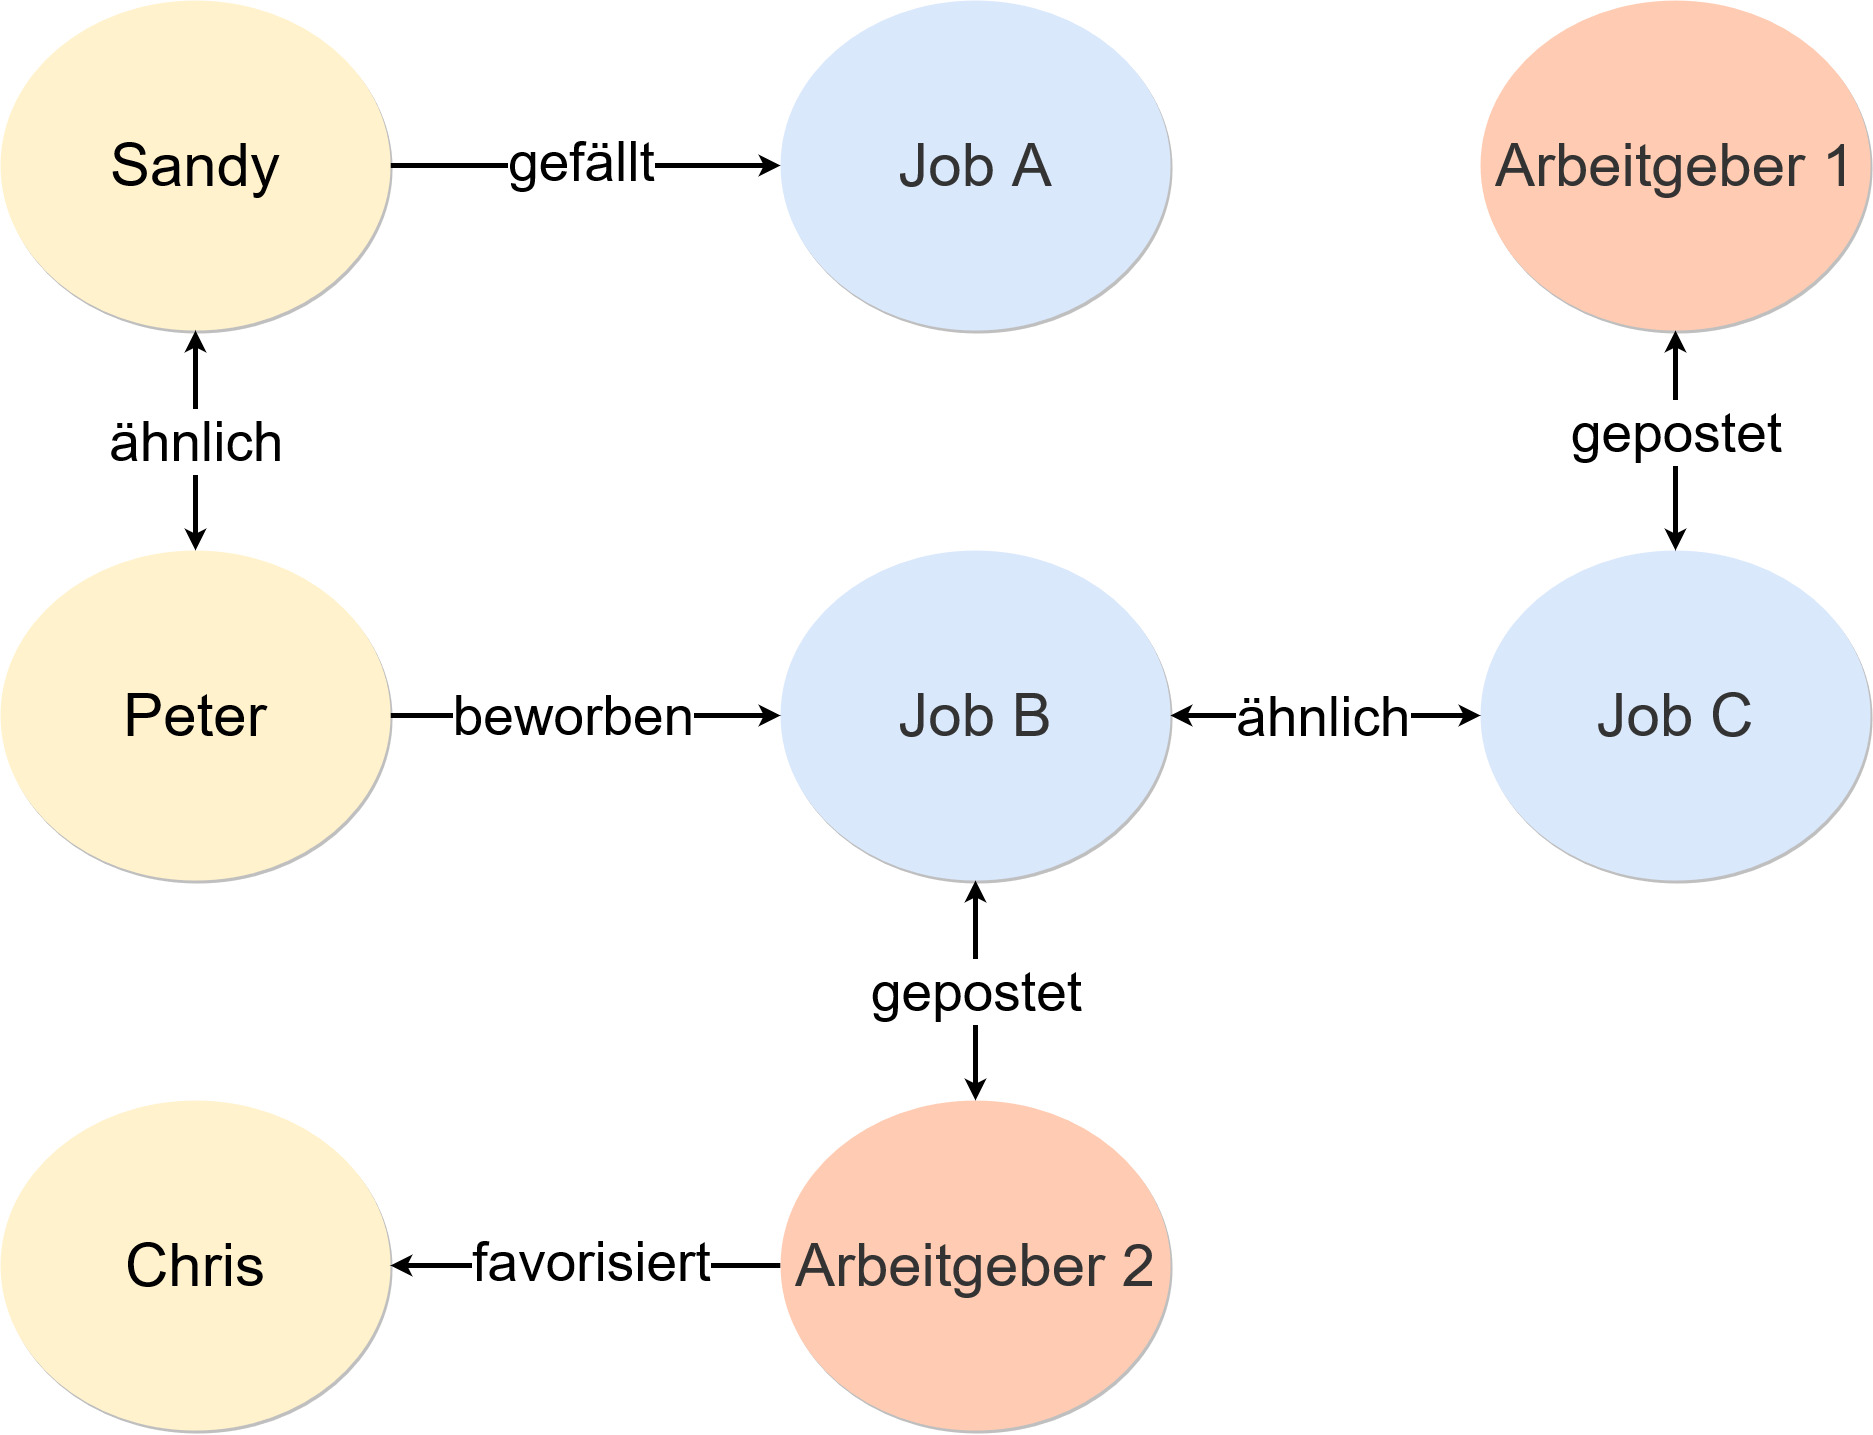
\includegraphics[width=0.9\textwidth]{gfx/lu-graph.jpg}
	\caption[Graphenstruktur des wechselseitigen Empfehlungssystems]{Graphenstruktur des wechselseitigen Empfehlungssystems\\
		(Eigene Darstellung in Anlehnung an \cite[S. 2]{lu:2013})}
	\label{fig:verwandteArbeiten:nichtAufDemPEFitBasierendeBilateraleSysteme:lu:2013:abb1}
\end{figure}

Kanten wurden im Graphen in Abbildung \ref{fig:verwandteArbeiten:nichtAufDemPEFitBasierendeBilateraleSysteme:lu:2013:abb1} für jede Interaktionen zwischen den Entitäten wie dem Besuch eines Profils oder dem Bewerben auf eine Stelle angelegt. Zusätzlich verfügte jede der dargestellten Entitäten über textuelle Profilbeschreibungen. Diese nutzten die Wissenschaftler als Grundlage für inhaltsbasierte Filterverfahren. Über diese bestimmten sie die Gleichartigkeit von Profilen und fügten bei hoher Ähnlichkeit zusätzliche Kanten in den Graphen ein. Über dieses Vorgehen behoben die Forscher die Problematik des Kaltstarts. Jede Kante im Graphen erhielt zudem ein bestimmtes Gewicht, sodass beispielsweise das Bewerben auf eine Stelle höher gewertet wurde als der Besuch eines Profils \cite[S. 1ff.]{lu:2013}.

Ein auf dem PageRank basierender Algorithmus unterstützte Stellensuchende und Arbeitgeber auf Grundlage des Graphen bei der Auswahl geeigneter Ausschreibungen bzw. Kandidaten. In die Berechnung wurde ein Personalisierungsfaktor einbezogen, welcher die Wichtigkeit der direkten Nachbarn eines Zielknotens erhöhte. In der finalen Ergebnisliste entfernte das System die direkten Nachbarn des Nutzers, um ausschließlich Elemente zu empfehlen, welche dem Anwender bislang unbekannt waren \cite[S. 3]{lu:2013}.

In einer Evaluation verglichen \textcite[S. 3f.]{lu:2013} die Genauigkeit ihres hybriden Systems mit den Ergebnissen des reinen kollaborativen und inhaltsbasierten Filterns. Hierbei stellten sie fest, dass ihr hybrider Empfehlungsansatz meist präzisere Ergebnisse liefern konnte als die beiden anderen Verfahren. Jedoch ist insbesondere bei der Empfehlung von Kandidaten für offene Stellen eine hohe Streuung in den Ergebnissen zu beobachten. So erzielte das hybride Empfehlungssystem bei dem Vorschlagen von Kandidaten für ein Stellenprofil eine Genauigkeit von 70 Prozent, während die inhaltsbasierte Recommender Engine lediglich 30 Prozent erzielte. Bei einem anderen Stellenprofil erreichte der hybride Ansatz dagegen nur eine Genauigkeit von 20 Prozent, während das inhaltsbasierte Verfahren 80 Prozent erzielte. Auf mögliche Ursachen dieser Abweichungen gingen \textcite[S. 1ff.]{lu:2013} nicht ein.

Kritisch muss außerdem festgestellt werden, dass die Autoren ihre Vorgehensweise zur Evaluation der Anwendung nicht erläuterten. Somit ist nicht feststellbar, ob das Empfehlungssystem auf Seiten der Kandidaten zu einer ausgeprägteren Zufriedenheit und aus Sicht der Unternehmen zu einer höheren Arbeitsleistung führte. Positiv sind die zahlreichen impliziten Bewertungen zu bemerken, welche \textcite[S. 1ff.]{lu:2013} verwendeten. Durch diesen Ansatz ist der zu erwartende manuelle Nutzeraufwand für die Pflege von Präferenzen sehr gering.
\shorthandon{"}
